\documentclass[tikz,border=5pt]{standalone}
\usepackage{pgfplots}
\pgfplotsset{compat=1.18}

\begin{document}
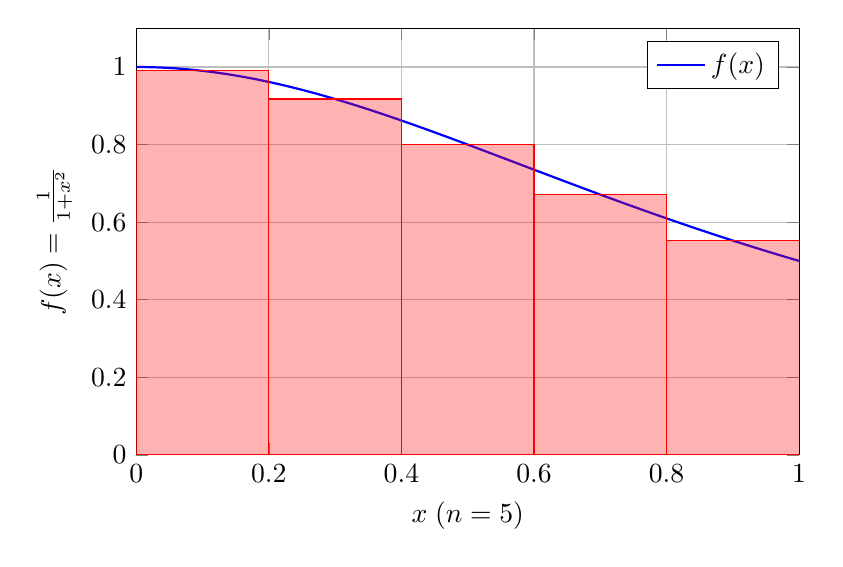
\begin{tikzpicture}
  \begin{axis}[
    xlabel={$x\; (n=5)$},
    ylabel={$f(x)=\frac{1}{1+x^2}$},
    xmin=0, xmax=1,
    ymin=0, ymax=1.1,
    grid=major,
    width=10cm,
    height=7cm,
    legend pos=north east
  ]
    \addplot[blue, smooth, thick, domain=0:1, samples=200] {1/(1+x^2)};
    \addlegendentry{$f(x)$}

    \addplot[red, fill=red, fill opacity=0.3, draw=red] 
        coordinates {(0,0) (0,0.9901) (0.2,0.9901) (0.2,0) (0,0)};
    \addplot[red, fill=red, fill opacity=0.3, draw=red] 
        coordinates {(0.2,0) (0.2,0.9174) (0.4,0.9174) (0.4,0) (0.2,0)};
    \addplot[red, fill=red, fill opacity=0.3, draw=red] 
        coordinates {(0.4,0) (0.4,0.8000) (0.6,0.8000) (0.6,0) (0.4,0)};
    \addplot[red, fill=red, fill opacity=0.3, draw=red] 
        coordinates {(0.6,0) (0.6,0.6711) (0.8,0.6711) (0.8,0) (0.6,0)};
    \addplot[red, fill=red, fill opacity=0.3, draw=red] 
        coordinates {(0.8,0) (0.8,0.5525) (1.0,0.5525) (1.0,0) (0.8,0)};
  \end{axis}
\end{tikzpicture}
\end{document}